\chapter{Preliminaries}

There are several preliminaries to this particular document, many of which are basic or rather facts regarding different notations, different theoretical knowledges, and so on, covering from mathematics of algebra to functional analysis, mathematical simulation and mathematical modelling, optimization theory and convergence bounds, concentration inequalities, coursework about computational theories, and so on. This will be condensed and precise, and does not aim to replace traditional knowledge or textbooks on such matter. For more information, please refer to authoritative sources as ideal. 
\section{Concentration inequalities}
A lot of results in statistical learning is proved using bounds. For example, if $X_{1},\dots,X_n$ are independent Bernoulli $(\theta)$ random variables representing the outcomes of a sequence of $n$ tosses of a coin with bias (probability of head), then for any $\epsilon \in (0,1)$: 
\begin{equation}\label{eqs:coin_toss_bound}
    \mathbb{P} \Big(\lvert \hat{\theta}_{n} - \theta \geq \epsilon\Big) \leq 2e^{-2\epsilon^{2}}, \quad \text{for } \hat{\theta}_{n} = \frac{1}{n} \sum^{n}_{i=1} X_i
\end{equation}
For the fraction of heads in $X^n=(X_1,\dots,X_n)$. Since $\theta = \mathbb{E}\hat{\theta}_{n}$, \ref{eqs:coin_toss_bound} says that the sample (or empirical) average of $X_{i}$ concentrates sharply around the statistical average. Bound like these are fundamental in statistical learning theory (well, mostly for proof, not going to lie). For now, let us learn the technique used to derive such bounds for settings much more complicated than coin tossing. 

\subsection{What are concentration inequalities?}

In a probabilistic setting, we are sometimes interested of the random fluctuations of functions of independent random variables. \textit{Concentration inequalities} quantify such statements, typically by bounding the probability that such a function differs from its expected value (or from its median) by more than a certain amount. 

The search for concentration inequalities has been a topic of intensive research in the last decades in a variety of areas because of their importance in numerous applications. Typically, this falls into the range of designing non-deterministic (by the definition of such words), dynamic randomized algorithms or procedure of interest, while able to bound them with concentration inequalities to a certain given degree of high probabilistic `accuracy', for example. Among the areas of applications, without trying to be exhaustive, we mention statistics, learning theory, discrete mathematics, statistical mechanics, random matrix theory, information theory, and high-dimensional geometry (while not actually sure why geometry is in here). 

Informally, the \textit{concentration phenomenon} asserts that if $X_{1},\dots,X_{n}$ are independent random variables, then $f(X_{1},\dots,X_{n})$ does not deviate much from its mean provided that $f(x_{1},\dots,x_{n})$ is not too sensitive in any of its coordinate $x_{i}$. While concentration properties for sums of independent random variables were thoroughly studied and fairly well understood in classical probability theory, powerful tools to handle more general functions of independent random variables were not introduced until the appearance of \textit{martingale methods} in the 1970s, by Yurinskii (1976), Maurey (1979), Milman and Schechtman (1986), Shamir and Spencer (1987) and McDiarmid (1989).
\begin{note}
    While the topic itself is much more complex than it is guaranteed to be, a \textit{martingale} can be defined as a sequence of random variables (i.e. for a stochastic process) for which, at a particular time, the conditional expectation of the next value in the sequence is equal to the present value, regardless of all prior values. A basic definition can be achieved. For a process $(M_n)_{n\geq 0}$, it is called martingale if:
    \begin{itemize}[noitemsep,topsep=1pt]
        \item For every $n\geq 0$, the expectation $\mathbb{E}[M_n]$ is finite, and hence equivalently, $\mathbb{E}[\lvert M_n \rvert]< \infty$.
        \item For every $n\geq 0$ and all $m_{n},m_{n-1},\dots,m_{0}$ we have: \begin{equation}
            \mathbb{E}(M_{n+1}\mid M_n = m_{n},\dots, M_{0}=m_{0}) = m_{n}
        \end{equation}
    \end{itemize} 
\end{note}

\subsection{Relevant toolset}
Of our book chapter, by a \textit{concentration inequality} we most often mean an upper bound for the probability that a real-valued random variable $Z$ differs from its expected value by more than a certain amount. In other word, we seek upper bounds for tail probabilities of the form 
\begin{equation}
    \mathbb{P}[Z-\mathbb{E}(Z)\geq t], \quad \mathbb{P}[Z-\mathbb{E}(Z)\leq -t] 
\end{equation}
where $t>0$. Of course, here we assume implicitly that the expected value exists, as for the probability to be included of the measurable space. 

To derive a lot of our concentration bounds that will solve such problem, however, we have to develop a few basic tools in the analysis. This will include Markov's inequality, Chebyshev's inequality, the Chernoff bound (often called the Chernoff trick), and Hoeffding's lemma. 
\subsection{Markov's inequality}
Let $Y\in \mathbb{R}$ be a nonnegative random variable. Then for any $t> 0$, we have the \textit{Markov's inequality} \index{Markov's inequality}: 
\begin{equation}
    \mathbb{P}(Y\geq t) \leq \frac{\mathbb{E}[Y]}{t}
\end{equation}
Before jumping straight into a proof, let us see what are we looking at from the perspective of the inequality.
%\begin{figure}[h!]
%    \centering
%    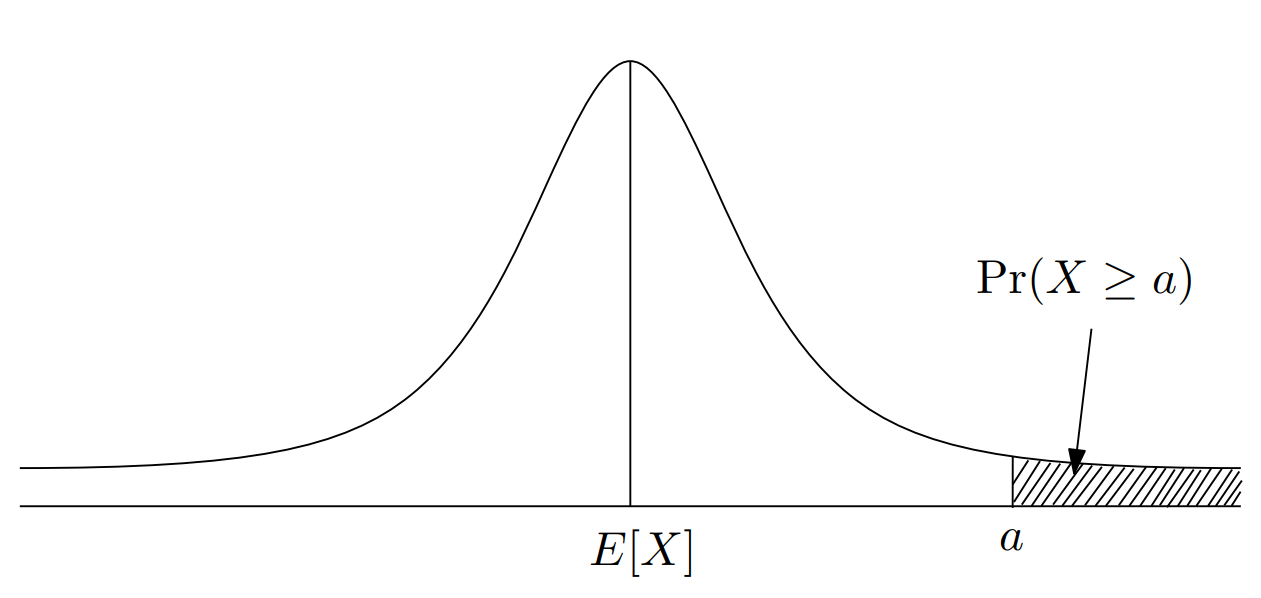
\includegraphics[width=0.7\textwidth]{img/markovbound.png}
%    \caption{Markov's inequality bounds the probability for the shaded region $\mathbb{P}[X\geq a]$}
%\end{figure}
\begin{proof}
    The proof is straightforward: \begin{equation}
        \begin{split}
            \mathbb{P}(Y\geq t) & = \mathbb{E}[\mathbbm{1}_{(Y\geq t)}]\\
            & \leq \frac{\mathbb{E}[Y\mathbbm{1}_{(Y\geq t)}]}{t}\\
            & \leq \frac{\mathbb{E}[Y]}{t}
        \end{split}
    \end{equation}
    We use the fact that\begin{equation}
        \mathbb{P}(Y\in A) = \int_{A} P_{Y} (dy) = \int_{Y} \mathbbm{1}_{(x\in A)} P_{Y}(dy) = \mathbb{E}[\mathbbm{1}_{Y\in A}]
    \end{equation}
    Additionally, we also have $Y\geq t > 0$ implies $Y/t \geq 1$, and $Y\geq 0\implies Y \mathbbm{1}_{(Y\geq t)}\leq Y$ which implies their expected value.
\end{proof}

If $\phi$ denotes a nondecreasing and nonnegative function defined on a possibly infinite interval $I\subset \mathbb{R}$, and if $Y$ denotes a random variable taking values in $I$, then Markov's inequality implies that for every $t\in I$ with $\phi(t)\neq 0$, 
\begin{equation}
    \mathbb{P} (Y\geq t) \leq \sP [\phi(Y)\geq \phi(t)] \leq \frac{\mathbb{E}[\phi(Y)]}{\phi(t)}
\end{equation}
This can be used to derive the Chebyshev's inequality later. 
\subsection{Chebyshev's inequality}
The common application of Markov's probability is Chebyshev's probability. Let $X$ be an arbitrary real random variable. Then for any $t> 0$, 
\begin{equation}
    \mathbb{P}(|X-\mathbb{E}[X]| \geq t) \leq \frac{\mathrm{Var}[X]}{t^{2}} 
\end{equation}
Where $\mathrm{Var}[X]:= \mathbb{E}[|X-\mathbb{E}X|^{2}]=\mathbb{E}[X^{2}]- (\mathbb{E}[X])^{2}$ is the variance of $X$. The prominent role of Chebyshev's inequality is not only explained by historical reasons, but also among all the absolute moments of the form $\mathbb{E}[|Z-\mathbb{E}(Z)|^{q}]$, the variance is typically the easiest to handle. 
\begin{proof}
    Let $X$ be a random variable, so $(X-\mathbb{E}[X])^{2}$ is a non-negative random variable. Hence, we can apply Markov's inequality: 
    \begin{align}
        \mathbb{P}(X-\mathbb{E}[X]\geq t) & = \mathbb{P}\left((X-\mathbb{E}[X])^{2}\geq t^{2}\right)\\
        & \leq \frac{1}{t^{2}} \mathbb{E} \left[(X-\mathbb{E}[X])^{2}\right]\\
        & = \frac{1}{t^2} \mathrm{Var}[X]
    \end{align}
\end{proof}
The property of Chebyshev's inequality contains several constraints, though arguably better than Markov's. Chebyshev's inequality does not require that the random variable is non-negative. However, it also requires that we know the variance in addition to the mean. Hence, the goal of Chebyshev's inequality is to bound the probability that the RV is far from its mean in either direction. While in principle Chebyshev's inequality asks about distance from the mean in either direction, it can still be used to give a bound on how often a random variable can take large values, and will usually give much better bound than Markov's inequality - since we have more knowledge of the distribution. 

We can use Chebyshev's inequality to prove a soft variation of the law of large number, or the \textit{weak law of large number}. 
\begin{theorem}[Weak Law of Large Number]
    Let $X_{1},\dots,X_{n}$ be a sequence of i.i.d. random variables with mean $\mu$. Let $\bar{X}_{n}=(1/n)\sum_{i=1}^{n}X_{i}$ be the sample mean. Then $\bar{X}_{n}$ converges in probability to $\mu$. That is, for any $\epsilon>0$, 
    \begin{equation}
        \lim_{n\to\infty}\mathbb{P}\left(\lvert \bar{X}_{n}-\mu\rvert > \epsilon\right)=0
    \end{equation}
\end{theorem}
\begin{proof}
    By the property of the expectation and variance of sample mean consisting of $n$ i.i.d. variables, for $\mathbb{E}[\bar{X}_{n}]=\mu$ and $\mathrm{Var}(\bar{X}_{n})=\sigma^{2}/n$. By Chebyshev's inequality, 
    \begin{equation}
        \lim_{n\to\infty} \mathbb{P}\left(\lvert \bar{X}_{n}-\mu\rvert > \epsilon\right) \leq \lim_{n\to \infty} \frac{\mathrm{Var}(\bar{X}_{n})}{\epsilon^{2}} = \lim_{n\to\infty} \frac{\sigma}{n\epsilon^{2}} = 0
    \end{equation}
    thus recover our desired equation. 
\end{proof}
\subsection{McDiarmid's inequality}
A generalization of Hoeffding's inequality is the McDiarmid's, or Bounded Difference inequality, where the quantity of interest is some function of the data, i.e. $S_{n}= \phi(X_{1},\dots,X_{n})$. Some restrictions on $\phi$ are required to get exponential bounds. 
\begin{theorem}[McDiarmid's Inequality]
    Let $X_{1},\dots,X_{n}$ be independent random variables, where $X_{i}$ has range $\mathcal{X}_{i}$. Let $f:\mathcal{X}_{1}\times \dots \times \mathcal{X}_{n}\to \mathbb{R}$ be any function with the $(c_1, \dots, c_{n})$-bounded difference property: for every $i=1,\dots,n$ and every $(x_1,\dots,x_n),(x_{1}',\dots,x_{n}')\in \mathcal{X}_{1}\times \dots\times \mathcal{X}_{n}$ that differ only in the $i$-th coordinate, we have: \begin{equation}
        \lvert f(x_1,\dots,x_n) - f(x_{1}',\dots,x_{n}') \rvert \leq c_{i}
    \end{equation}
    For any $t>0$: 
    \begin{equation}
        \mathbb{P}\Big([f(X_{1},\dots,X_{n})] - \mathbb{E}[f(X_{1},\dots,X_{n})]\geq t\Big) \geq \exp{\left(-\frac{2t^{2}}{\sum_{i=1}^{n}c_{i}^{2}}\right)}
    \end{equation}
\end{theorem}
\begin{proof}
    Write $\mathbb{E}_i[\cdot]$ to denote expectation conditioned on $X_{1:i} := (X_1, \ldots, X_i)$. Therefore, $g_i(X_{1:i}) := \mathbb{E}_i[f(X_{1:n})]$ is, as the notation suggests, a function of $X_{1:i}$. Now define the following random variables:
\[
Y_i := g_i(X_{1:i}) - g_{i-1}(X_{1:i-1}),
\]
\[
A_i := \inf_{x_i \in \mathcal{X}_i} g_i(X_{1:i-1}, x_i) - g_{i-1}(X_{1:i-1}),
\]
\[
B_i := \sup_{x_i \in \mathcal{X}_i} g_i(X_{1:i-1}, x_i) - g_{i-1}(X_{1:i-1}).
\]

These random variables satisfy
\[
Y_i \in [A_i, B_i], \quad \mathbb{E}_{i-1}[Y_i] = 0,
\]
\[
\sum_{i=1}^n Y_i = f(X_{1:n}) - \mathbb{E}[f(X_{1:n})].
\]

Furthermore, we claim that $[A_i, B_i]$ is always an interval of length at most $c_i$. We defer the proof of this claim to later.  

To bound the probability that the sum of the $Y_i$'s is at least $t$, we use the Chernoff bounding method. Let $S_i := Y_1 + \cdots + Y_i$. Then
\begin{align}
    \mathbb{E}[\exp(\lambda S_n)] 
    &= \mathbb{E}[\exp(\lambda(Y_n + S_{n-1}))] \\
    &= \mathbb{E}[\mathbb{E}_{n-1}[\exp(\lambda Y_n)] \exp(\lambda S_{n-1})]\\
    &\leq \exp(\lambda^2 c_n^2/8)\,\mathbb{E}[\exp(\lambda S_{n-1})]\\
    &= \exp(\lambda^2 c_n^2/8)\,\mathbb{E}[\exp(\lambda(Y_{n-1}+S_{n-2}))]\\
    &= \exp(\lambda^2 c_n^2/8)\,\mathbb{E}[\mathbb{E}_{n-2}[\exp(\lambda Y_{n-1})]\exp(\lambda S_{n-2})]\\
    &\leq \exp(\lambda^2 c_n^2/8)\exp(\lambda^2 c_{n-1}^2/8)\,\mathbb{E}[\exp(\lambda S_{n-2})]\\
    & \vdots \\
    &\leq \exp(\lambda^2 c_n^2/8)\cdots\exp(\lambda^2 c_1^2/8) \\
    &= \exp\left(\frac{\sum_{i=1}^n c_i^2}{4}\cdot\frac{\lambda^2}{2}\right).
\end{align}

Above, the inequalities all follow from Hoeffding's inequality. Therefore, $S_n$ is $\sum_{i=1}^n c_i^2/4$ sub-Gaussian. The probability bound now follows from the Cramer-Chernoff inequality for subgaussian random variables.

It remains to prove that $[A_i, B_i]$ is an interval of length at most $c_i$. We show that $B_i - A_i \leq c_i$. By independence of $X_1, \ldots, X_n$, we have

\begin{align}
g_i(X_{1:i-1}, x_i) 
&= \mathbb{E}[f(X_{1:i-1}, x_i, X_{i+1:n}) \mid X_{1:i-1}, X_i = x_i]   \\
&= \mathbb{E}[f(X_{1:i-1}, x_i, X'_{i+1:n}) \mid X_{1:i-1}],  
\end{align}
where $X'_{i+1:n}$ is an independent copy of $X_{i+1:n}$. Then
\begin{align}
B_i - A_i 
&= \sup_{b \in \mathcal{X}_i} g_i(X_{1:i-1}, b) - \inf_{a \in \mathcal{X}_i} g_i(X_{1:i-1}, a)   \\
&= \sup_{a,b \in \mathcal{X}_i} g_i(X_{1:i-1}, b) - g_i(X_{1:i-1}, a)  \\
&= \sup_{a,b \in \mathcal{X}_i} \mathbb{E}[f(X_{1:i-1}, b, X'_{i+1:n}) - f(X_{1:i-1}, a, X'_{i+1:n}) \mid X_{1:i-1}]   \\
&\leq \mathbb{E}\Big[\sup_{a,b \in \mathcal{X}_i} |f(X_{1:i-1}, b, X'_{i+1:n}) - f(X_{1:i-1}, a, X'_{i+1:n})| \,\Big|\, X_{1:i-1}\Big]   \\
&\leq c_i.  
\end{align}

The last step above uses the bounded differences property of $f$.
\end{proof}

\subsection{The Cramer-Chernoff method}
One more important bounding method that can be discussed in this section is the Cramer-Chernoff bound. This method determines the best possible bound for a tail probability that one can possibly obtain by using Markov's inequality with an exponential function $\phi(t)=\exp{(\lambda t)}$. This simple technique leads to surprisingly sharp bounds in many cases. We work out some simple examples, and then will proceed with some of its analytical properties. 

Let $Z$ be a real-valued random variable. For $\lambda\geq 0$, Markov's inequality implies 
\begin{equation}
    \sP [Z\geq t] \leq \exp{(-\lambda t)}\mathbb{E}[\exp{(\lambda Z)}]
\end{equation}
Since this inequality holds for all values of $\lambda \geq 0$, one may choose $\lambda$ to minimize the upper bound. Defining the logarithm of the moment generating function as 
\begin{equation}
    \phi_{Z}(\lambda) = \log{(\mathbb{E}[\exp{(\lambda Z)}])}, \quad \forall \lambda \geq 0 
\end{equation}
and introducing the supremum of such generating function being \begin{equation}
    \phi_{Z}^{*}(t) = \sup_{\lambda\geq 0}(\lambda t - \phi_{Z}(\lambda))
\end{equation}
We obtain the Chernoff's inequality:\index{Chernoff's inequality} 
\begin{equation}
    \sP [Z\geq t] \leq \exp{\left[-\left(\sup_{\lambda\geq 0}(\lambda t - \phi_{Z}(\lambda))\right)\right]} = \exp{[-\phi_{Z}^{*}(t)]}
\end{equation}
The function $\phi_{Z}^{*}(t)$ is called the \textit{Cramer transform} of $Z$. Usually, this is also called the Legendre transform (for example, in \cite{OstaszewskaZajkowski2014}) or Legendre-Fenchel transform. The Cramer transform is characterized of its shape by satisfying the \textit{Cramer's condition},\index{Cramer condition} 
\begin{definition}[Cramer's condition]
    Let $M_{X}$ denote the moment-generating function of a given random variable $X$, that is, $M_{X}(t)=\mathbb{E}[\exp{(tX)}]$. Then the random variable $X$ satisfies the \textit{Cramer condition} if there exists $c>0$ such that $\mathbb{E}[\exp{(|cX|)}]< \infty$. If $X$ satisfies the Cramer condition, then we call $M_{X}$ to be \textit{well-defined} (taking finite values) on a connected neighbourhood, containing the interval $[-c,c]$, of zero and moreover possess the expansion
    \begin{equation}
        M_{X}(t) = \sum^{\infty}_{n=0}\frac{\mathbb{E}[X^{n}]}{n!}t^{n}
    \end{equation}
    where $|t|<t_{0}$ and $t_{0}>c$. 
\end{definition}
The function itself is a nonnegative function, since $\phi_{Z}(0)=0$. If $\mathbb{E}[Z]$ exists, then the convexity of the exponential function and Jensen's inequality imply that $\phi_{Z}(\lambda)\geq \lambda \mathbb{E}[Z]$ and therefore, for all negative values of $\lambda$, $\lambda t - \phi_{Z}(\lambda)\leq 0$ whenever $t\leq \mathbb{E}[Z]$. This means that we may formally extend the supremum over all $\lambda \in \mathbb{R}$ of the Cramer transform, 
\begin{equation}
    \phi_{Z}^{*}(t) = \sup_{\lambda\in \mathbb{R}}(\lambda t - \phi_{Z}(\lambda))
\end{equation}
from this, formally, we treat the right-hand expression of the often known, as what we call the \textit{Fenchel-Legendre dual function} of $\phi_{Z}$. Thus, at every $t\geq \mathbb{E}[Z]$, the Cramer transform coincides with the Fenchel-Legendre dual. That is not to say they are the same, however the range of $\lambda$ is relevant. 

\section{Metric and pseudometric}

One of the treatment, or rather insight that we would be looking at, consider the notion of a \textbf{metric}. Of those, we think of it as an additional structure upon two sets, to encode specific quantization to the notion of distinguishability, and distance metric. Out of those, there are the space of such admissible constructions, which includes \textit{metric space} and \textit{pseudometric spaces}. 

\begin{definition}[Pseudometric space]
    Suppose $X$ is a set. A function $\rho: X\times X \to \mathbb{R}$ is said to be a \textbf{pseudometric}, if it satisfies:
    \begin{enumerate}[itemsep=1pt,topsep=1pt,label=\roman*]
        \item $\rho(x,x)=0$, $\forall x\in X$, 
        \item $\rho(x,y)=\rho(y,x)$, $\forall x,y\in X$,
        \item $\rho(x,z)\leq \rho(x,y)+\rho(y,z)$, $\forall x,y,z\in X$. 
    \end{enumerate}
    The value of $\rho$ is positive-bounded, such that we can write $\rho:X\times X\to \mathbb{R}_{+}$. Suppose $\rho$ is a pseudometric on $X$, then we say that $(X,\rho)$ is a \textbf{pseudometric space}.
\end{definition}

We can see that a pseudometric would not impose characteristic on distinguishment upon two points, but only identifiability via $\rho(x,x)$. In fact, if two points are of zero-distance on the metric $\rho$, such cannot be determined if the two points are the same, but rather only a weaker form of $x\sim y$ as to require $\rho(x,y)=0$. If, however, we impose that they are the same, then we gain a metric. 
\begin{definition}[Metric]
    Suppose $X$ is a set. A function $\rho^{*}: X\times X \to \mathbb{R}$ is said to be a \textbf{metric} if it is a pseudometric, and satisfies $\rho^{*}(x,y)=0\Rightarrow x=y$. Then, we say $(X,\rho^{*})$ is a \textbf{metric space}.
\end{definition}

Later on, we would be seeing the difference between the two, and one of the categorical error of choosing metric space condition on loss-functional space. Let us illustrate the construction for now in this section. Let $\mathcal{H}$ be the hypothesis class of arbitrary structure, $\mathcal{Z}$ the admitted observations space, $\ell :\mathcal{H}\times \mathcal{Z}\to \mathbb{R}_{+}$ as the loss functional or resultant loss application on $\mathcal{H}\times \mathcal{Z}$, and suppose there exists a quantification of probability distribution $\mathcal{P}$ on $\mathcal{Z}$ of which we suppose to capture generating patterns on the observation pack. Then, the error functional on admitted dataset most often is of the form similar to an empirical error measure,
\begin{equation}
    \hat{R}(h) = \underset{z\sim \mathcal{P}}{\mathbb{E}} [\ell(h,z)]
\end{equation}
and thus giving us, suppose that there exists the $\mathcal{A}$-algorithm that produces $h_{i},h_{i+1},\dots$, the following distance metric:
\begin{equation}
    d_{\ell} (h_{i},h_{i+1}) := \underset{z\sim \mathcal{P}}{\mathbb{E}} \Big[ | \ell(h_{i},z) - \ell(h_{i+1},z) | \Big]
\end{equation}
This object satisfies \textit{non-negativity}, \textit{symmetry}, and \textit{triangle inequality} as specified of pseudometric. However, often we do not have the virtue to say that if $d_{\ell}(h_{i},h_{i+1})=0$ then $h_{i}=h_{i+1}$, aside from which we have total exposure of the system itself. Let us consider the setting. Suppose that for the picture $(z,\mathcal{P})$ of the perceived observations space characteristic, it has a true concept $c\in\mathcal{C}$ of arbitrary structure concept class $\mathcal{C}$. For any assumption on oracle access on $c$, we see that $R(c)\leq 0$ take as arbitrary $\epsilon$, since observation can deviate from the concept resultant observation itself. Hence, we get that 
\begin{equation}
    \begin{split}
        d(h_{i},c) := \underset{z\sim \mathcal{P}}{\mathbb{E}} \Big[ | \ell(h_{i},z) - \ell(c,z) | \Big] &\leq \underset{z\sim \mathcal{P}}{\mathbb{E}} [\ell(h_{i},z)] + \underset{z\sim \mathcal{P}}{\mathbb{E}} [\ell(c,z)] \\
        & = \underset{z\sim \mathcal{P}}{\mathbb{E}} [\ell(h_{i},z)] + \epsilon
    \end{split}
\end{equation}
which means that even by this, the distance is never guaranteed as to be zero. And that is within oracle access setting itself. Usually, if this is not guaranteed, then we have no access on $c$, thus we also have no access to complete this distance metric calculation on itself, and thus $d(h,c)$ does not exist. Here is the conflation of the effect. If, we are to assume that we are comparing the notion of $x=y$ for any object of the functional space itself as to be the factorization, or parameterization that governs $z\to q$ of the input-output observable space on $\mathcal{Z}$, then the loss-functional gives a metric, as for $d(h,c)=0$ means they phenomenologically approach the same focal point. However, if the target is structural, then $d(h,c)=0$ does not mean $h=c$, even by assumption that $\mathcal{H}=\mathcal{C}$ i.e. concept space and the hypothesis space has same scope. Putting that aside, because we never have access to $c$, the way to interpret, with presumption of $c$ to exist, then $\ell(h,z)=\ell(c,z)$ only guarantees that we settle the model is an equivalence class $h\sim c$ only; this is strengthened if we further consider that $(\mathcal{Z},\mathcal{P})$ imposes a structural proxy $c^{*}$ that can deviate from $c$, and can also admit different structural interpretation outside of class $\mathcal{C}$. Thereby, interpretively, loss-functional space is not metric but pseudometric, when it comes to the target $c$ measure in which the measure comparing to this object simply does not exist. To obtain equality, one typically use quotient space on it, which is a very strong structural addition and assumption, and might, or might not, be guaranteed, though in this direction of admitting quotient decision space is valid. If, however, one approaches the other way, by saying that different hypotheses must be metrically distinguishable, i.e. imposing injectivity on $\ell$, full support on distribution $\mathcal{P}$, and identifiability condition, that the assumption set would be very strong and almost never work in practice. 

\section{Graph theory}

We retain a section explicitly about graph theory, partially because it would be used as a provisional example in the material, specifically in experimental setting. Thereby, we would like to contain several trivializations of knowledge on such structure. 

\begin{definition}[Graph]
    A \textbf{simple graph} is a pair $(V,E)$, where $V$ is a finite set, and where $E$ is a subset of $\mathcal{P}_{2}(V)$, with $\mathcal{P}_{2}(V)$ is the set of all 2-element subsets of $V$.
\end{definition}

A quick way to refers to certain elements of the graph is as followed.

\begin{definition}[Notations]
    Let $G=(V,E)$ be a simple graph. 
    \begin{enumerate}[itemsep=1pt,topsep=1pt]
        \item The set $V$ is the vertext set of $G$, denoted $\mathrm{V}(G)$. The element of $V$ are called the \textbf{vertices} (or \textbf{nodes}) of $G$. 
        \item The set $E$ is called the \textbf{edge set} of $G$, denoted $\mathrm{E}(G)$. The element of $E$ are called the \textbf{edges} of $G$.  We denoted $uv$ for $\{u, v\}$ as connections between $u$ adn $v$.
    \end{enumerate}
\end{definition}

Certain properties of such simple graph case follows: 

\begin{definition}[Connectedness]
    If the two graphs are $G_{1}=(V(G_{1}),E(G_{1}))$ and $G_{2}=(V(G_{2}),E(G_{2}))$ where $V(G_{1})$ and $V(G_{2})$ are disjoint, then their \textbf{union} $G_{1}\cup G_{2}$ is the graph with vertex set $V(G_{1})\cup V(G_{2})$ and edge family $E(G_{1})\cup E(G_{2})$. 
\end{definition}

\begin{definition}[Adjacency]
    Two vertices $u,v$ are said to be \textbf{adjacent} to each other if $wv\in E$. $uv$ is then said to \textbf{join} $u$ with $v$. The \textbf{neighbour} of a vertex $v\in V$ is then the set of all $u\in V$ such that $uv\in E$. 
\end{definition}

\begin{definition}[Graph Isomorphism]
    Let $G$ and $H$ be two simple graphs. A \textbf{graph isomorphism} (or \textbf{isomorphism}) from $G\to H$ is the bijection $\phi: \mathrm{V}(G)\to \mathrm{V}(H)$ that \textit{preserves edges}, i.e., for any two vertices $u$ and $v$ of $G$, we have \begin{equation}
        (uv \in \mathrm{E}(G)) \iff (\phi (u)\phi (v) \in \mathrm{E}(H))
    \end{equation} We say that $G$ and $H$ are isomorphic (denoted $G \cong H$) if there exists a graph isomorphism from $G$ to $H$. 
\end{definition}

We also list several types of graphs, specifically, the \textbf{subgraph}, null /complete graph, path /cycle graph, Kneser graphs, diagraphs and multigraph (or general graph).\todo[author=Amane,fancyline]{What if, for a general graph, there are \textbf{multiple non-equal edges and connections}, such that each node function more as a small subgraph, or either an itermediate I/O node?} 

\begin{definition}[Subgraph]
    A subgraph of a graph $X$ is a graph $Y$ such that $\mathrm{V}(Y)\subseteq \mathrm{V}(X)$ and $\mathrm{E}(Y)=\mathrm{E}(X)$. If $\mathrm{V}(Y) = \mathrm{V}(X)$ then $Y$ is a \textit{spanning subgraph} of $X$. A subgraph $Y$ of $X$ is an \textit{induced subgraph} if two vertices of $\mathrm{V}(Y)$ are adjacent in $Y$ if and only if they are adjacent in $X$. 
\end{definition}

One of the important definition for subgraph, especially for those of recommendation system, and graph construction network, is the notion of \textbf{induced subgraph}. 
\begin{definition}[Induced subgraph]
    Let $S\subset V$. The induced subgraph of $G$ on the set $S$ denotes the subgraph \begin{equation}
        (S, E\cap \mathcal{P}_2 (S))
    \end{equation}
    of $G$. In other words, it denotes the subgraph of $G$ whose vertices are the elements of $S$, and whose edges are precisely those edges of $G$ whose both endpoints belong to $S$. 
\end{definition}

\begin{definition}[Null graph]
    A graph whose edge-set $E=\varnothing$ is a \textbf{null graph}. we denote the null graph on $n$ vertices by $N_{n}=(V,\varnothing)$. 
\end{definition}

\begin{definition}[Complete graph]
    A simple graph $G=(V,E)$ in which each pair of distinct vertices are adjacent is a \textbf{complete} graph. We denote this by $K_{n}$. For graph $K$ with $\mathrm{V}(G)= n$, we have: \begin{equation}
        V(K_n) = \frac{n(n-1)}{2}
    \end{equation}
\end{definition}

\begin{definition}[Path graph]
    For each $n\in \mathbb{N}$, we define the $n$-th \textbf{path graph} $P_n$ to be the simple graph \begin{equation}
        P_n = (\{1,2,\dots,n\, \{ i(i+1) \mid 1 \leq i < n \})
    \end{equation}
    This graph has $n$ vertices and $n-1$ edges (unless $n=0$)
\end{definition}

\begin{definition}[Cycle graphs]
    For each $n>1$, we define the $n$-th \textbf{cycle graph} $C_n$ to be the simple graph \begin{equation}
        C_n = (\{1,\dots,n\}, \{ i(i+1) \mid 1 \leq i < n \} \cup \{1n\} )
    \end{equation}
    This graph has $n$ vertices and $n$ edges, unless $n=1$, then it has only 1 edge. For multigraph, however, the $C_2$ graph can have two edges. 
\end{definition}


\subsection{Algebraic representation}
The tool of computation is still linear algebra, for any large computational system under the neural network system. Hence, there are several useful way to represent such graph on linear algebraical notation and system. 
\begin{definition}[Adjacency matrix]
    Let $G$ be a simple graph with $V(G)=\{1,\dots,n\}$ and $E(G)= \{e_1, \dots, e_m\}$. The adjacency matrix of $G$, denoted $A(G)$, is the $n\times n$ matrix defined as \begin{equation}
        A_{dj} = A \in \mathbb{R}^{n\times n}: \quad A_{ij} = \begin{cases}
            1 & v_i v_j \in E, i \neq j \\
            0 & \text{ otherwise}
        \end{cases}
    \end{equation}
\end{definition}

The modification (somewhat familiar) of the adjacency matrix is by the notion of \textbf{incidence matrix}, which takes into account the case of directed graph.
\begin{definition}[Incident matrix]
    Let $G$ be a graph with $\mathrm{V}(G)=\{1,\dots,n\}$ and $\mathrm{E}(G)=\{e_1,\dots,e_m\}$. Suppose each edge $e\in \mathrm{E}(G)$ is an orientation, which is arbitrary but fixed. The (vertex-edge) \textbf{incidence matrix} of $G$, denoted $Q(G)$, is the matrix of size $n\times m$, defined as followed: 
    \begin{equation}
        Q(G) \in \mathbb{R}^{n\times m} : \quad Q_{ij} = \begin{cases}
            1 & (i, e_j)\in G, e_j \text{ originates at } i\\
            -1 & (i, e_j)\in G, e_j \text{ terminates at } i\\
            0 & \text{ otherwise (both)}
        \end{cases}
    \end{equation}
    For undirected graph, the matrix is defined as 
    \begin{equation}
        Q(G) \in \mathbb{R}^{n\times m} : \quad Q_{ij} = \begin{cases}
            1 & \exists k, e_j = \{v_i, v_k\}\\
            0 & \text{ otherwise}
        \end{cases}
    \end{equation}
\end{definition}

For multidirected graph (or multigraph), we use the \textbf{Laplacian matrix} to represent such graph in matrix form. Notice that of the coming definition, the Laplacian matrix does not encode incidences in its matrix, as it is not the main focus of the definition. 
\begin{definition}[Laplacian matrix]
    Let $G$ be a graph with $\mathrm{V}(G)=\{1,\dots,n\}$ and $\mathrm{E}(G)=\{e_1,\dots,e_m\}$. The \textbf{Laplacian matrix} of $G$, denoted $L(G)$, is the $n\times n$ matrix defined as followed: 
    \begin{equation}
        L(G)\in \mathbb{R}^{n\times m} : L_{ij} = \begin{cases}
            0 & i \neq j \\
            deg(i) & i = j
        \end{cases}
    \end{equation}
\end{definition}

The Laplacian matrix and the incidences matrix can be related, with the fixed orientation assumption, by \begin{equation}
    L(G) = Q(G)Q'(G)
\end{equation} where $Q'(G)$ is the transpose of $Q$. This identity suggests that the Laplacian might depends on the orientation, although it is evident from the definition that the Laplacian is independent of orientation. 


We present more subsidiary theory on graph theory. 
\begin{theorem}[Handshaking Lemma]
  In any graph $G$, the sum of all the vertex-degree is an even number. Or, the vertex degree add up to \textit{twice} the number of edges: $$\sum_{v\in V(G)}\mathrm{deg}_{G}(v)= 2\lvert E(G) \rvert $$
\end{theorem}
\begin{proof}[Proof by induction]
  The base case here is $m=0$. The graph with no edge then $\mathrm{deg}(v)=0$. 

Assume that the degree sum formula holds for all $(m-1)$-edge graphs. Let $G$ be a graph with $m\geq 1$ edges, and let $xy$ be any edge of $G$. We can apply the inductive hypothesis to $G-xy$ (the graph we get from \textbf{deleting} $xy$ from $G$), a graph with $m-1$ edges. 

Both $x$ and $y$ have one extra incident edge in $G$ they don't have in $G-xy$ - the edge $xy$ itself. Hence $$\mathrm{deg}_{G}(x)=1+\mathrm{deg}_{G-xy}(x)$$
and $$\mathrm{deg}_{G}(y)=1+\mathrm{deg}_{G-xy}(y)$$
For any other vertex $v$, $G-xy$ and $G$ have the same number of edges, so we have $$\mathrm{deg}_{G}(v)=\mathrm{deg}_{G-xy}(v)$$
Furthermore, $G-xy$ and $G$ have the same set of vertices. So if we add up the vertex degrees in $G-xy$ and $G$, the result is that $$\sum_{v\in V(G)} \mathrm{deg}_{G}(v)= 2+ \sum_{V\in V(G-xy)}\mathrm{deg}_{G-xy}(v)$$
Applying the inductive hypothesis, we get that the degree sum in $G-xy$ is $2(m-1)$, so the degree sum in $G$ is $2(m-1)+2=2m$. By induction, the degree sum formula holds all graphs.  
\end{proof}

\subsection{Permutation invariance and equivariance}

In mathematical terms, any function $f$ that takes an adjacency matrix $\mathbf{A}$ as input should ideally satisfy one of the two following properties: 
\begin{align}
  f(\mathbf{PAP})^{\top}= f(\mathbf{A})\quad \text{(Permutation Invariances)}\\
  f(\mathbf{PAP^{\top}}) = \mathbf{P}f(\mathbf{A})\quad \text{(Permutation Equivariance)}
\end{align}
where $\mathbf{P}$ is a permutation matrix. Permutation invariance means that the functin does not depend on arbitrary ordering of the rows/coulmns in the adjacency matrix, while permutation equivariance means that the output of $f$ is permuted in a consistent way when we permute the adjacency matrix. 

\subsection{Graph Fourier Transform}

In graph theory, especially for the \textbf{spectral graph theory}, we present an encoding standard, called the \textbf{graph Laplacian}. Then we will focus on the Fourier analysis of such grpah representation, such as the \textit{graph Fourier transform}. For the purpose, however, we believe that the spectral graph theory alongside its analysis can get us to the layered encoding appropriated of analysing the aggregation contour that the graph is taken into. 
\subsubsection{Graph Laplacian}
Given the adjacency matrix $A\in \{0,1\}^{n\times n}$ and degree matrix $D\in \mathbb{Z}^{n\times n}$, for a graph $G=(V,E)$, we define the graph Laplacian as the matrix $L$ such that: \begin{equation}
  L:= D- A
\end{equation}

Intuitively, it is the analog for the Laplacian operator $\Delta f(x)= \nabla\cdot \nabla f(x)$. In this form, it is quite different from the above Laplacian matrix, but the same idea applies. In this form, it is perhaps better for analysis, though. 

We list several conclusive properties of the Laplacian matrix: 
\begin{enumerate}[itemsep=1pt,topsep=1pt]
  \item $L$ is a real symmetric matrix, there by $\lambda_k > 0, \forall \lambda \in \{\lambda_k\}_{k=0}^{N-1}$ with associated orthornomal eigenvectors $\{\varphi_k\}^{N-1}_{k=0}$.
  \item If $G$ is finite and connected, then \begin{equation}
    0= \lambda_0 < \lambda_1 < \dots < \lambda_{N-1}
  \end{equation}
  \item The spectrum of the Laplacian $\sigma(L)$ is fixed but one's choice of eigenvectors $\{\varphi_k\}^{N-1}_{k=0}$ can vary. Throughout the paper, we assume that the choice are fixed. 
  \item Let $\Psi$ denote the $N\times N$ matrix where the $k$-th column is precisely the vector $\varphi_k$, then we can easily show that $\varphi_0 = 1/\sqrt{N}$. 
\end{enumerate}

\subsubsection{Fourier transformation}

Let $G(V,E)$ be a weighted graph, $\mathbf{L}$ be its corresponding graph Laplacian, and $f: V\to \mathbb{R}$ a function defined on the vertices of $G$. The \textbf{Graph Fourier Transform} (GFT) is defined as
\begin{equation}
  \mathcal{GF}[f](\lambda_{l}) = \hat{f}(\lambda_{l}) = \langle f, \varphi_{l} \rangle = \sum_{i=1}^{n} f(i) \varphi_{l}(i)
\end{equation}

The inverse Fourier transform is then given by \begin{equation}
  f(n) = \sum_{i=0}^{N-1} \hat{f}(\lambda_{l})\varphi_{l}(n) 
\end{equation}

This also leads it to the graph convolution (used in graph convolutional network) as
\begin{equation}
  f * g(n) = \sum_{l=0}^{N-1} \hat{f}(\lambda_{l})\hat{g}(\lambda_l)\varphi_{l}(n)
\end{equation}
for $f,g: V\to \mathbb{R}$ as functions on the continuous domain. 
